\documentclass{article}
\usepackage[UTF8]{ctex}  % 使用中文支持包
\usepackage[a4paper, margin=1in]{geometry}  % 设置纸张大小和边距
\usepackage{anyfontsize}  % 解决字体大小报错问题
\usepackage{fancyhdr}  % 设置页眉、页脚、页码
\usepackage{longtable}  % 支持长表格

\usepackage{amsmath}  % 数学公式支持
\usepackage{cases}  % 支持联立编号

\usepackage{graphicx}  % 插入图片支持
\usepackage{float}  % 设置图片浮动位置
\usepackage{subfigure}  % 插入多图时用子图显示

\usepackage{listings}  % 代码块支持
\usepackage{xcolor}  % 设置代码块颜色

\usepackage[hyphens]{url}  % 支持链接换行
\usepackage{hyperref}  % 超链接支持
\usepackage{lastpage}  % 添加lastpage包
\usepackage{gbt7714}  %国标参考文献
\bibliographystyle{gbt7714-numerical}
\hypersetup{
    hidelinks,
    colorlinks=true,
    allcolors=black,
    pdfstartview=Fit,
    breaklinks=true
}

\title{射线源导论-第一次小测}
\author{\LaTeX\ by\ Jerry\ }
\date{\today}
\pagenumbering{arabic}

\begin{document}
\pagestyle{fancy}

\fancyhead[L]{Jerry}
\fancyhead[C]{射线源导论-第一次小测}
\fancyhead[R]{\today}
\fancyfoot[C]{Page \thepage/\pageref{LastPage}}

\section*{第一次小测}

\subsection*{1. (4分)}

\emph{直线轨迹 $a-b-c$ 是一个束团运动的参考轨道,$a$ 和 $b$ 点分别是一个无限薄聚焦透镜的人射和出射表面位置,该透镜的焦距为 $f$,$c$ 点距离透镜为 $f$ ,如图 1 所示。一个束团在 $a$ 点的相空间分布如图 2(a)所示,$x’$ 方向宽度可忽略($x'=\frac{p_x}{P_z}$),$x$方向最大最小值分别为 $D$ 和$-D$,束团被透镜聚焦后达到 $b$ 点,之后在不受任何外力或自场力作用情况下漂移到 $c$ 点。请在图 2(b)和(c)中分别画出 $b$、$c$点位置的束团相空间,并标注出分布离中心最远处两点的坐标。}

\begin{figure}[htbp]
    \centering
    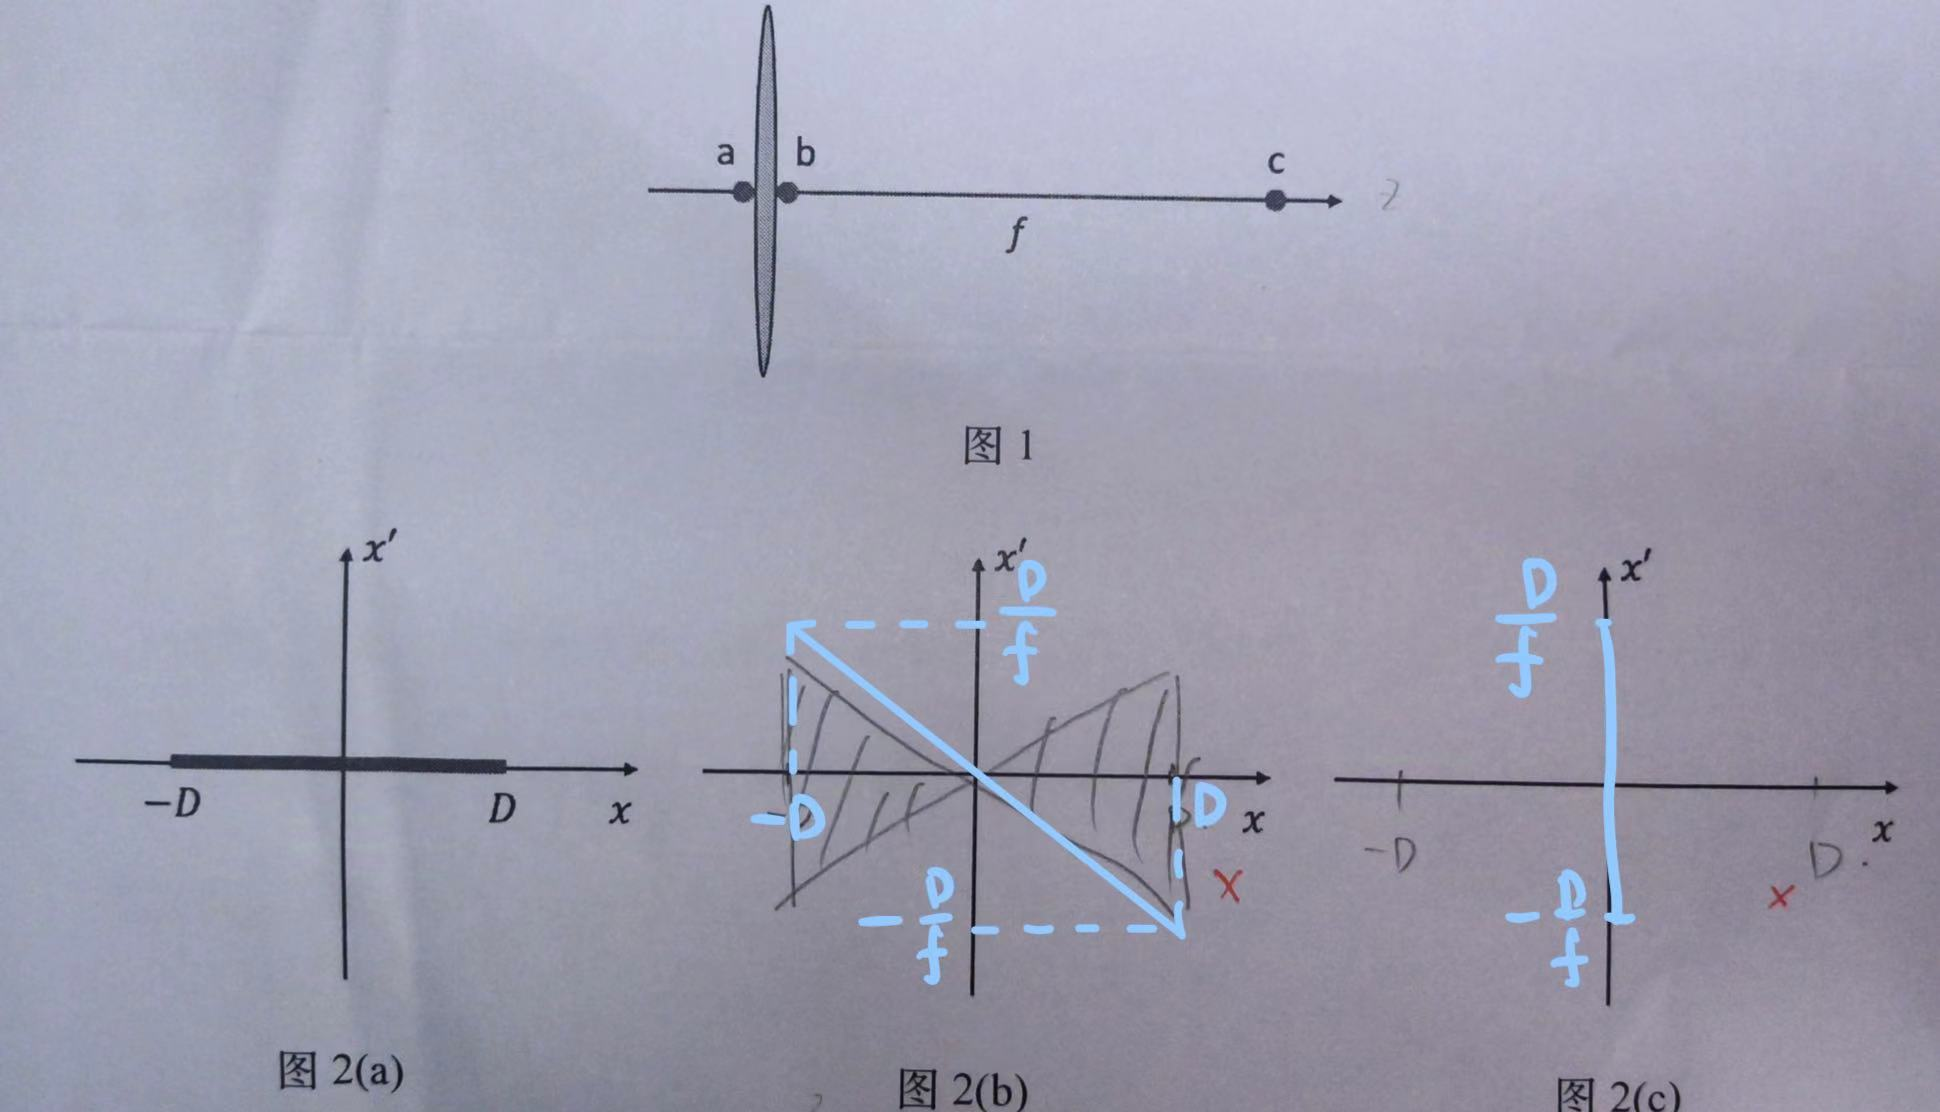
\includegraphics[width=0.8\textwidth]{./img/1.jpg}
    \caption{题目图示}
    \label{fig:1}
\end{figure}

\subsection*{2. (2分)}

\emph{动能为 1 GeV 的缪介子(muon)的洛伦兹因子是\_\_\_\_\_\_?其波长是\_\_\_\_\_\_。}

首先,缪介子的静止质量 $ m $ 大约为 105.7 MeV/c²。动能 $ T $ 为 1 GeV

洛伦兹因子 $\gamma = \frac{E}{m c^2}$

总能量 $$E = T + m c^2 = 1000 \, \text{MeV} + 105.7 \, \text{MeV} = 1105.7 \, \text{MeV}$$

所以洛伦兹因子 $ \gamma $ 为:

$$\gamma = \frac{1105.7 \, \text{MeV}}{105.7 \, \text{MeV}} \approx 10.46$$

德布罗意波长公式:

$$\lambda = \frac{h}{p}$$

由 $ E = 1105.7 \, \text{MeV} $,$ m c^2 = 105.7 \, \text{MeV} $,有:$$p c \approx 1101.4 \, \text{MeV}$$

计算波长:$$\lambda = \frac{h c}{p c} = \frac{1240 \text{eV}, \text{nm}}{1101.4 \times 10^6 \, \text{eV}} \approx 1.24 \times 10^{-15} \, \text{m}$$

\subsection*{3. (3分)}

\emph{设计一支采用六硼化镧阴极的热阴极电子枪,要求电子枪发射的最小电流密度为$1A/mm^2$,试计算阴极需达到的最低温度是多少$K$?如果阴阳极均为平板结构且面积足够大,阴阳极之间间隙$2cm$,阴阳极之间加载的电压值应超过为多少伏?六硼化镧($LaB_6$)的功函数$W$为$2.70eV$,$A*b$系数为$29$}

理查德逊-劳德曼方程:$$J = A T^2 e^{-\frac{W}{kT}}$$

其中 $J$ 为电流密度,$A$ 为常数,$T$ 为温度,$W$ 为功函数,$k$ 为玻尔兹曼常数。

代入数据:$$1 = 29 \times T^2 \times e^{-\frac{2.70}{8.617 \times 10^{-5} \times T}}$$

解得$ T = 2211K $

$$J = \frac{4}{9} \varepsilon_0 \sqrt{\frac{2e}{m_e}} \frac{V_0^{3/2}}{d^2} = 1A/mm^2$$

解得 $V_0 = 3.09\times10^5V$

\subsection*{4. (3分)}

\emph{线性光电发射过程中,吸收光子的被激发电子的发射过程受哪些因素影响?能发射出来的激发电子运动方向与材料表面法线方向的夹角$\theta_{max} $ 与哪些参数相关?}

\begin{itemize}
    \item 金属内电子吸收光子的吸收率 $1-R(W)$
    \item 电子在金属表面不被另一个电子散射概率 $F_{e-e}$
    \item 金属表面状况、金属表面形状、功函数、光强、光频率
\end{itemize}

$$\theta_{max}^{in}=\arccos\frac{\sqrt{E_f+\phi_{eff}}}{\sqrt{E+\hbar\omega}}$$

故与有效功函数、光子能量、费米能级、电子能级有关

\subsection*{5. (3分)}

\emph{某种光阴极材料的功函数是$4.2eV$,那么能够从该材料表面激发线性光电效应的最长激光波长为\_\_\_\_\_\_ . 如果再在该材料表面施加$100MV/m$的加速场,则有效功函数变为\_\_\_\_\_\_}

由$\nu = \frac{E}{h} = \frac{1}{\lambda}$, 有$$\lambda = \frac{1240}{4.2} \approx 295.43$$

对于$100MV/m$的加速场,由第三周作业可知,势垒降低$V_x = 0.379eV$

故有效功函数为$3.821eV$

\end{document}
